% Chapter 2

\chapter{Traducción de problemas NP}
\label{Chapter2}
\lhead{Capítulo 2. \emph{Traducción de problemas NP}}
Este capítulo describe el diseño de una herramienta capaz de transformar una
descripción de un problema en lógica de segundo orden existencial
en un problema de planificación perteneciente a la clase de complejidad
equivalente (NP).
Primero se explica el funcionamiento a alto nivel de la herramienta, en función
de sus entradas y salidas. Luego, se define formalmente una función de
traducción de lógica a planificación, demostrando las propiedades pertinentes.
Finalmente, se presenta la gramática de un lenguaje de especificación basado en lógica 
y se describe brevemente la implementación de la herramienta, que consiste en un 
analizador sintáctico y función de traducción ya descrita.

\section{Perspectiva general}
Como puede verse en la Figura \ref{esquema_herramienta}, la herramienta tiene
como entradas una sentencia $\Phi\in\SOE(\sigma)$, y
una estructura finita de primer orden $\A\in\struc[\sigma]$ sobre la cual se
intentará probar la propiedad definida por $\Phi$.
Las salidas son un dominio y una instancia PDDL que tienen un plan válido si y
sólo si $\A$ satisface $\Phi$. Además, un \textbf{certificado} de la validez de
la propiedad en $\Phi$ puede obtenerse del plan en tiempo lineal.

\begin{figure}[h]
\centering
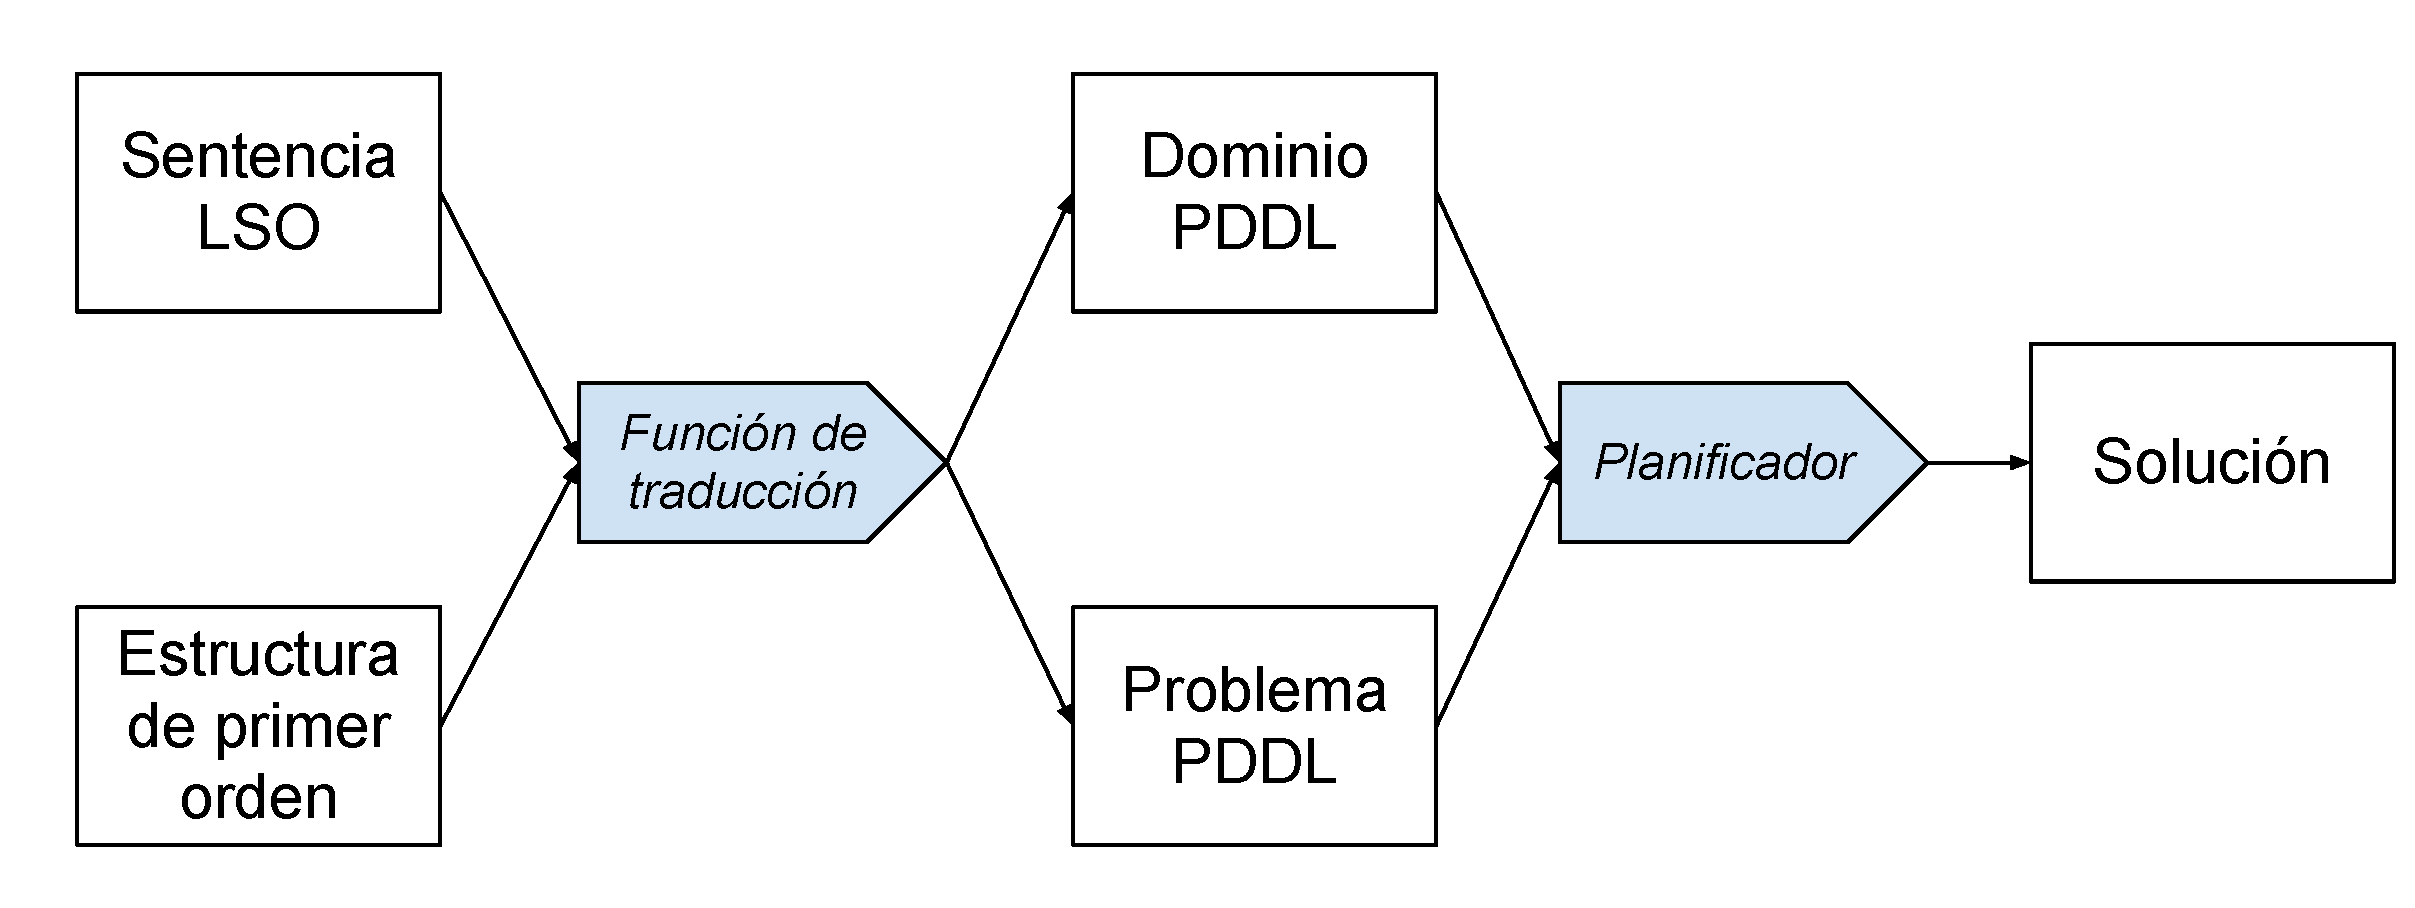
\includegraphics[width=\textwidth]{figuras/esquema_herramienta.pdf}
\caption{Esquema de operación de la herramienta}
\label{esquema_herramienta}
\end{figure}

La traducción se basa en convertir la tarea de demostrar la validez de la
fórmula lógica en una tarea de planificación. Por lo tanto, las acciones del
dominio de planificación harán las veces de las operaciones de semántica
formal, probando cada tipo de subfórmula según un esquema similar a la
definición \ref{semantica_def}. La información específica al problema, como el
estado inicial, está codificada por la estructura de primer orden que recibe la
herramienta. Se ha visto que estas estructuras pueden representar grafos, por lo
que el \textit{software} es especialmente útil para la modelación y resolución
de problemas de grafos.

Desde el punto de vista del usuario, la contribución de esta herramienta es
proveer una forma alternativa y descriptiva de especificar problemas de forma
que sea posible obtener e interpretar su solución.


Hence, we can think of the tool as a generator of reductions
among problems. Recall that, in general, a reduction from problem
$A$ into problem $B$ is a computable function $f$ such that
for each instance $\omega$, $\omega\in A$ iff $f(\omega)\in B$.

In our case, the reduction decomposes in two functions
\begin{alignat*}{1}
&\domred: \text{Signatures} \times \SOE \rightarrow \text{PDDL Domains}\,, \\
&\insred: \text{Signatures} \times \SOE \times \struc \rightarrow \text{PDDL Instances}
\end{alignat*}
such that $\domain=\domred(\sigma,\Phi)$ is a PDDL domain
and $\instance=\insred(\sigma,\Phi,\A)$ is an instance.

In order to get something of theoretical and practical 
interest, the reduction should run in polynomial time,
so that it would not be able to check whether $\A$
satisfies $\Phi$ and then produce a trivial planning
problem, and its output should be solvable in NP so that
complexity of solving the output problem is no bigger than
solving the input problem.
However, the plan-existence decision problem for PDDL is
not in NP because (1)~the number of grounded fluents
and actions may be exponential in the input size, and
(2)~a minimum-length plan may be of exponential size in
the number of grounded fluents and actions.
Thus, not every reduction qualifies for our purposes
and we must be careful with its design. In the following
two sections, we present an acceptable reduction and 
study its formal properties.

\section{Reducción de LSO a STRIPS}
\subsection{Reducción del dominio}
\subsection{Reducción del problema}

\section{Propiedades formales}
Las propiedades más importantes a considerar en la herramienta son solidez,
completitud y garantía de complejidad. Que la función de traducción sea sólida
y completa significa que ella realmente implementa una reducción entre problemas de
decisión, mientras que la garantía de complejidad se refiere al tiempo
requerido para computar la reducción y la complejidad de decidir la existencia
de un plan en el problema generado. En esta sección se demuestra que la 
herramienta es una reducción en tiempo
polinomial del problema NP expresado por $\Phi$ a un fragmento de planificación
que es decidible en NP.

%! ???
Considere la función de \emph{instanciación} $\ground$ que transforma el par
$\tup{\domain,\instance}$ de un dominio y problema PDDL en un problema STRIPS
$P = \ground(\domain, \instance)$. Para un $\domain$ fijo, la función
$\instance\leadsto\ground(\domain, \instance)$ corre en un tiempo polinomial
$\O(\|\instance\|^k)$ para algún $k$ que sólo depende de $\domain$; de hecho,
$k$ es la máxima aridad de un predicado o acción en el dominio.

De manera similar, la función de traducción $\insred$ corre en tiempo
polinomial en el tamaño de la estructura $\A$, pero exponencial sobre la aridad
más grande de un cuantificador de segundo orden existencial en $\Phi$. De este
modo, la función $f_{\sigma,\Phi}:\struc[\sigma]\rightarrow\text{STRIPS}$
definida por 
\[ f_{\sigma,\Phi}(\A) = \ground(\domred(\sigma,\Phi),\insred(\sigma,\Phi,\A)) \]
es una función en tiempo polinomial que asigna a las $\sigma$-estructuras un
problema instanciado STRIPS.

Se debe demostrar que la función $f_{\sigma,\Phi}(\A)$ es una reducción y que
los problemas de planificación que produce tienen a lo sumo la misma
complejidad que \SOE.

\subsection{Demostración de reducción}
Se demostrará que $\A \models \Phi$ si y sólo si $f_{\sigma,\Phi}(\A)$ tiene
solución, es decir, si y sólo si existe un plan que alcanza $\FT[\Phi]$ desde
el estado inicial (que depende de $\A$).

\begin{proposition}
\label{t1}
Sean $t_1,\ldots,t_k$ términos instanciados, es decir, que no contienen
variables. Sea $\A$ una estructura, $u\in|\A|$ y `$a$' una constante tal que
$a^\A=u$.
Entonces, $(\A, i[x:=u]) \models \varphi(t_1,\ldots,t_k,x)$ si y sólo si
$(\A, i) \models \varphi(t_1,\ldots,t_k,a)$.
\end{proposition}
\begin{proof}
Directa de la definición de verdad.
\end{proof}
\begin{corollary}
\label{corolario}
Sean $t_1,\ldots,t_k$ términos instanciados. Sea $\A$ una
estructura en donde todos los objetos tienen nombre (i.e., para todo $u\in|\A|$
existe una constante $a$ tal que $a^\A=u$). Entonces,
$(\A, i) \models (\exists x) \varphi(t_1,\ldots,t_k,x)$ si y sólo si
existe una constante `$a$' tal que $(\A, i) \models \varphi(t_1,\ldots,t_k,a)$.
\end{corollary}
\begin{theorem}
Sea $\varphi \in \LPO(\sigma)$ y $t_1,\ldots,t_k$ $\sigma$-términos instanciados. Sea $\A \in
\struc[\sigma]$ tal que todo objeto tiene nombre y sea $i : \text{VAR} \longrightarrow |\A|$.
Entonces, $(\A, i) \models \varphi(t_1,\ldots,t_k)$ si y sólo si
existe un plan $\pi[t_1,\ldots,t_k]$ que alcanza
$\FT[\varphi](t_1,\ldots,t_k)$ desde el \textbf{estado inicial} $S[\A]$,
donde $S[\A]$ es el estado de STRIPS definido por las siguientes condiciones:
\begin{alignat*}{1}
& S[\A] = \{\texttt{prueba}\} \cup \{ \texttt{R}(a_1,\ldots,a_k) :
\tup{a_1^\A,\ldots,a_k^\A} \in R^\A\}\\
& {\color{white} S[\A] = } \cup \{\texttt{no-R}(a_1,\ldots,a_k) : \tup{a_1^\A,\ldots,a_k^\A} \not\in R^\A\}\\
& {\color{white} S[\A] = } \cup \{\texttt{SUC}(a_i, a_{i+1}) : 0 \leq i < n\}
\end{alignat*}

\end{theorem}
\begin{proof}
Hacemos la demostración por inducción sobre la estructura de $\varphi$. El caso
base corresponde a las fórmulas atómicas de la forma $\varphi =
R(t_1,\ldots,t_k)$:
\begin{alignat*}{1}
& \quad \quad (\A, i) \models \varphi(t_1,\ldots,t_k)\\
& \iff \tup{\text{definición \ref{semantica_def}(b)}} \\
& \quad \quad \tup{t_1,\ldots,t_k} \in R^\A\\
& \iff \tup{\text{definición de S[\A]}}\\
& \quad \quad \texttt{R}(t_1,\ldots,t_k) \in S[\A]\\
& \iff \tup{\text{definición de } \FT}\\
& \quad \quad \FT[\varphi](t_1,\ldots,t_k) \in S[\A]\\
& \iff \tup{\text{el plan vacío alcanza la condición } \FT[\varphi](t_1,\ldots,t_k)}\\
& \quad \quad \pi[t_1,\ldots,t_k] =\ \tup{} \textbf{ es el plan.}
\end{alignat*}
El caso $\varphi = \neg R(t_1,\ldots,t_k)$ es análogo al anterior, con
\texttt{not-R}$(t_1,\ldots,t_k) \in S[\A]$ en lugar de \texttt{R}$(t_1,\ldots,t_k)$.
Ahora consideramos las fórmulas más complejas:

Caso $\varphi = \varphi_1(t'_1,\ldots,t'_{k'}) \land \varphi_2(t_1'',\ldots,t''_{k''}) $:
\begin{alignat*}{1}
& \quad \quad (\A, i) \models \varphi(t_1,\ldots,t_k)\\
& \iff \tup{\text{definición \ref{semantica_def}(d)}}\\
& \quad \quad (\A, i) \models \varphi_1(t'_1,\ldots,t'_{k'}) \text{ y } 
(\A, i) \models \varphi_2(t''_1,\ldots,t''_{k''})\\
& \iff \tup{\text{hipótesis inductiva}}\\
& \quad \quad \pi_1[t'_1,\ldots,t'_{k'}] \text{ y } 
\pi_2[t_1'',\ldots,t''_{k''}] \text{ son planes que alcanzan }\\
& \quad \quad \FT[\varphi_1](t'_1,\ldots,t'_{k'}) \text{ y } \FT[\varphi_2](t'_1,\ldots,t'_{k''})
\text{ desde } S[\A]\\
& \iff \langle \text{como no hay \textit{deletes}, aplicar ambos planes en
secuencia }\\
& {\color{white}\iff\langle} \text{garantiza alcanzar
$\FT[\varphi](t_1,\ldots,t_k)$ desde $S[\A]$} \rangle\\
& \quad \quad \textbf{el plan }\tup{\pi_1(t'_1,\ldots,t'_{k'});\
\pi_2(t_1'',\ldots,t_{k_2}'');\ \texttt{probar\_y\_}\varphi(t_1,\ldots,t_k)} \\
& \quad \quad \textbf{alcanza la condición }
\FT[\varphi](t_1,\ldots,t_k) \textbf{ desde } S[\A]
\end{alignat*}

Caso $\varphi = \varphi_1(t_1',\ldots,t'_{k_1}) \lor \varphi_2(t''_1,\ldots,t''_{k_2}) $:
\begin{alignat*}{1}
& \quad \quad (\A, i) \models \varphi(t_1,\ldots,t_k)\\
& \iff \tup{\text{definición \ref{semantica_def}(e)}}\\
& \quad \quad (\A, i) \models \varphi_1(t'_1,\ldots,t'_{k'}) 
\text{ o } (\A, i) \models \varphi_2(t''_1,\ldots,t''_{k''})\\
& \text{Por casos. Caso $(\A, i) \models \varphi_1(t'_1,\ldots,t'_{k'})$:}\\
& \quad \iff \tup{\text{hipótesis inductiva}}\\
& \quad \quad \quad \pi_1[t_1,\ldots,t_{k_1}] \text{ es un plan que alcanza 
$\FT[\varphi_1](t_1,\ldots,t_{k_1})$ desde $[\A]$}\\
& \quad \iff \langle \text{no hay \textit{deletes}} \rangle\\
& \quad \quad \textbf{el plan } \tup{\pi_1(t_1,\ldots,t_{k_1});\
\texttt{probar\_o\_}\varphi(t_1,\ldots,t_k)} \\
& \quad \quad \textbf{alcanza la condición }
\FT[\varphi](t_1,\ldots,t_k) \textbf{ desde } S[\A]\\
& \text{Caso $(\A, i) \models \varphi_2(t''_1,\ldots,t''_{k''})$:}\\
& \quad \quad \text{Análogo al caso anterior.}
\end{alignat*}

Caso $\varphi = \varphi_1(t_1',\ldots,t'_{k'}) \Rightarrow \varphi_2(t''_1,\ldots,t''_{k''}) $:

\quad Ver caso anterior, pues $\varphi_1 \Rightarrow \varphi_2 = \neg \varphi_1 \lor \varphi_2$.

Caso $\varphi = (\exists x)\ \theta(t_1,\ldots,t_k,x):$
\begin{alignat*}{1}
& \quad \quad (\A, i) \models \varphi\\
& \iff \langle \text{por corolario \ref{corolario}, ya que todo objeto en $|\A|$
tiene nombre, }\\
& {\color{white} \iff \langle} \text{ existe una constante } `a' \rangle\\
& \quad \quad (\A, i) \models \theta(t_1,\ldots,t_k,a)\\
& \iff \tup{\text{hipótesis inductiva}}\\
& \quad \quad \pi[t_1,\ldots,t_k,a] \text{ es un plan que alcanza }
\FT[\theta](t_1,\ldots,t_k,a) \text{ desde } S[\A]\\
& \iff \tup{\text{no hay \textit{deletes}}}\\
& \quad \quad \textbf{el plan } \langle \pi[t_1,\ldots,t_k,a];\
\texttt{probar\_existencial\_}\varphi(t_1,\ldots,t_k)\rangle\\
& \quad \quad \textbf{alcanza la condición } \FT[\varphi](t_1,\ldots,t_k)
\textbf{ desde } S[\A]
\end{alignat*}

Caso $\varphi = (\forall x)\ \theta(t_1,\ldots,t_k,x):$
\begin{alignat*}{1}
& \quad \quad (\A, i) \models \varphi\\
& \iff \tup{\text{definición \ref{semantica_def}(h), y todo objeto tiene nombre}}\\
& \quad \quad (\A, i) \models \theta(t_1,\ldots,t_k,a), \text{ para toda
constante $a$}\\
& \iff \tup{\text{hipótesis inductiva}}\\
& \quad\quad \text{para toda constante $a$ existe un plan $\pi[t_1,\ldots,t_k,a]$ que}\\
& \quad\quad \text{alcanza $\FT[\theta](t_1,\ldots,t_k,a)$ desde } S[\A]\\
& \iff \langle \text{existe un orden $a_i < a_{i+1}$ para todas las constantes,}\\
& {\color{white} \iff \langle} \text{ determinado por \texttt{SUC}, y no hay
\textit{deletes}} \rangle\\
& \quad \quad \textbf{el plan } \langle \pi_0[t_1,\ldots,t_k,a_0];\
\texttt{probar\_universal\_base\_}\varphi(t_1,\ldots,t_k);\\
& \quad \quad \pi_1[t_1,\ldots,t_k,a_1];\
\texttt{probar\_universal\_inductivo\_}\varphi(t_1,\ldots,t_k,a_1);\\
& \quad \quad \ldots\ \\
& \quad \quad \pi_{n-1}[t_1,\ldots,t_k,a_{n-1}];\
\texttt{probar\_universal\_inductivo\_}\varphi(t_1,\ldots,t_k,a_{n-1}) \rangle\\
& \quad \quad \textbf{alcanza la condición } \FT[\varphi](t_1,\ldots,t_k)
\textbf{ desde } S[\A]
\end{alignat*}
\end{proof}

\begin{theorem}
Sea $\Phi = (\exists R_1)\cdots(\exists R_n) \varphi$.
$\A \models \Phi$ si y sólo si existe un plan $\pi$ que alcanza $\FT[\Phi]$ desde $S[\A]$.
\end{theorem}
\begin{proof}
Por definición, $\A \models \Phi$ si y sólo si
$\tup{\A, R_1',\ldots,R_n'} \models \varphi$.
La hipótesis inductiva es que existe un plan $\pi'$ que alcanza $\FT[\varphi]$ a partir de $S[\A,
R_1',\ldots,R_n']$.
Basta mostrar que es posible alcanzar el estado $S[\A, R_1',\ldots,R_n']$ desde
$S[\A]$. Sea $u_j = a_j^\A$ para $1 \leq j \leq k$.
\begin{alignat*}{1}
& \textbf{El plan }\\
& \langle \ \tup{\texttt{colocar\_verdadera\_R\_i}(a_1,\ldots,a_{k_i}) 
\text{ para cada } \tup{u_1,\ldots,u_k} \in R_i} \text{ para cada } R_i \ ;\\
& {\color{white} \langle \ } \tup{\texttt{colocar\_falsa\_R\_i}(a_1,\ldots,a_{k_i}) \text { para cada
} \tup{u_1,\ldots,u_k} \not\in R_i} \text{ para cada } R_i\ ;\\
& {\color{white} \langle \ } \texttt{comenzar\_prueba}()\ \rangle\\
& \textbf{alcanza el estado } S[\A, R_1',\ldots,R_n'] \textbf{ desde } S[\A].
\end{alignat*}
\end{proof}

\subsection{Demostración de complejidad}
Como se ha mencionado en la sección \ref{complejidad_planificacion}, 
se sabe que verificar la existencia de un plan para 
problemas de planificación
sin efectos negativos está en NP \citep{bylander:plan-complexity}. La prueba
depende del hecho de que un plan óptimo no necesita repetir acciones, y por lo
tanto es de tamaño lineal. Puede extenderse esta noción: si todas las acciones que
agregan efectos negativos pueden ser aplicadas a lo sumo una vez, verificar la
existencia de un plan sigue estando en NP, pues el tamaño del plan no podrá ser
mayor al número de acciones.

\begin{definition}
Un problema de planificación $P = \tup{C, A, I, F}$ es de tipo
\textit{máximo-1} si y sólo si las acciones pueden ser particionadas en $A =
A_0 \cup A_1$, donde:
\begin{itemize}
\item Ninguna de las acciones de $A_0$ tiene efectos negativos, es decir,
$(\forall a \in A_0) (del(a) = \emptyset)$.
\item Todas las acciones de $A_1$ tienen una precondición que no es añadida por
ninguna acción, y que es borrada apenas $a$ es ejecutada, es decir, 
$(\forall aa' \in A_1)\ (\exists p \in pre(a) \cap del(a))\ (p \not\in add(a'))$
\end{itemize}

El conjunto de todos los problemas \textit{máximo-1} se denota como STRIPS-1.
\end{definition}

\begin{theorem}
Para toda estructura $\A$, $f_{\sigma, \Phi}(\A)$ es un problema STRIPS-1.
\end{theorem}
\begin{proof}
Ninguna de las acciones de $f_{\sigma, \Phi}(\A)$ tienen \textit{deletes} excepto
\texttt{comenzar\_prueba} y las acciones \texttt{colocar\_verdadera} y
\texttt{colocar\_falsa}, pero todas estas borran una precondición que no es
añadida por ninguna otra acción (i.e., pertenecen a $A_1$ según la definición
de STRIPS-1).
\end{proof}

\begin{theorem}
El problema de decisión de existencia de un plan STRIPS-1 es NP-completo.
\end{theorem}
\begin{proof}
\ \\ \textbf{Inclusión:} Todas las acciones de $A_1$ pueden ser aplicadas a lo
sumo una vez. Como estas acciones pueden borrar condiciones (tienen
\textit{deletes}), en el peor caso puede requerirse aplicar \textbf{todas} las
acciones de $A_0$ antes de aplicar otra acción de $A_1$. Por lo tanto, el
tamaño de un plan es a lo sumo cuadrático en el número total de acciones.
\\ \textbf{Dificultad:} $f_{\sigma_{\textsc{SAT}}, \Phi_{\textsc{SAT}}}$ reduce SAT a STRIPS-1 en
tiempo polinomial.
\end{proof}

Por lo tanto, la herramienta traduce cualquier problema NP, codificado con una
sentencia \SOE, a STRIPS-1.

\section{Diseño del lenguaje}

\subsection{Gramática}
\begin{alignat*}{1}
\sofbf\   & \deriv\ \lpar \SOExists\ \lpar \listrel \rpar\ \sofbf \rpar \\
          & \deriv\ \lpar \SOForall\ \lpar \listrel \rpar\ \sofbf \rpar \\
          & \deriv\ \pofbf \\[1em]
\listrel\ & \deriv\ \rel\ \integer\ \listrel\ |\ \rel\ \integer \\
          & \deriv\ \rel\ \tipof\ \listrel\ |\ \rel\ \tipof\ \\[1em]
\tipof\   & \deriv\ \fun\ |\ \pfun\ |\ \inj\ |\ \pinj\ \\[1em]
\pofbf\   & \deriv\ \lpar \rel\ \listvar \rpar \\
          & \deriv\ \lpar \NOT\ \pofbf \rpar \\
          & \deriv\ \lpar \AND\ \listpofbf \rpar \\
          & \deriv\ \lpar \OR\ \listpofbf \rpar \\
          & \deriv\ \lpar \IMPLIES\ \pofbf\ \pofbf \rpar \\
          & \deriv\ \lpar \Exists\ \lpar \listvar \rpar\ \pofbf \rpar \\
          & \deriv\ \lpar \Forall\ \lpar \listvar \rpar\ \pofbf \rpar \\[1em]
\listvar\ & \deriv\ \var\ \listvar\ |\ \var \\[1em]
\end{alignat*}


%\begin{theorem}
%La función $f_{\sigma, \Phi}$ es una reducción en tiempo polinomial del
%problema de decisión inducido por $\Phi$ a STRIPS-1.
%\end{theorem}
%
%\begin{proof}
%Se quiere demostrar que
%$\A\models(\exists R_1^{a_1})\cdots(\exists R_k^{a_k})\psi$ si y sólo si
%existe un plan que consigue la condición $\FT[\psi]$. La prueba es inductiva
%sobre la estructura de la sentencia de primer orden $\psi$. Se demostrará que para toda subformula 
%$\theta$ de $\psi$, y toda interpretacion $(\\A,i)$ de $\A$:
%
%\[ (\\A,i) \models \theta(\overline{X}) \iff \text{existe un plan para } \FT[\theta](\overline{X}) \]
%
%Por implicación mutua. Primero se prueba
%\[ (\\A,i) \models \theta(\overline{X}) \Rightarrow \text{existe un plan para } \FT[\theta](\overline{X}) \]
%\end{proof}
